\documentclass[11pt]{article}

%%% Useful packages
\usepackage{graphicx}

%%% Sets page margins, overriding 11pt article defaults
\setlength{\topmargin}{0 in}
\setlength{\headheight}{0 in}
\setlength{\headsep}{0 in}
\setlength{\oddsidemargin}{0in}
\setlength{\textwidth}{6.5 in}
\setlength{\textheight}{9 in}

%%% Useful for layout
\newcommand{\VF}{\vspace*{\fill}}
\newcommand{\HF}{\hspace*{\fill}}

\begin{document}

\noindent {\large \textbf{Math 4107, Fall 2021, Homework 0}}
\bigskip
\bigskip

%%% Edit the file below.  Two sample answers have been given.
%%% A blank line starts a new paragraph.  '\\' is a line break.   
%%% The default formatting is usually acceptable, so don't spend 
%%% a significant amount of time making your solutions look pretty.  
%%% Do spellcheck.  PROOFREAD, more than once!

\noindent Registration name: \\
Sean Eva
\bigskip

\noindent Name you wished to be called in class: \\
Sean
\bigskip

\noindent gtID\#: 903466156	\\

\noindent (3 points) Provide a recent, clearly recognizable image of yourself: \\
%%% Does not have to be done in latex for full credit.  Just leave enough 
%%% space using \hspace*{3in} command, print out PDF, attach an image
%%% by hand, and upload to Gradescope.

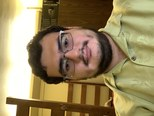
\includegraphics{me4.jpg}

\noindent Major(s) and target graduation date: I am majoring in Math and I plan to graduate Spring 2023\\

\noindent At least one reason why you chose the field(s) of study that you did: I really enjoyed math related activities in high school such as things like math team and tutoring students. Additionally, I knew I wanted to go into a STEM field but not what in specific, so I chose to major in math so that I have a lot of opportunities for what I can do in the future.\\


\noindent List your last three math classes, including professor and semester (and institution if not Tech): 
\begin{enumerate}
    \item MATH 3406: Linear Algebra 2, Igor Belegradek
    \item MATH 3235: Probability Theory, Federico Bonetto
    \item MATH 2106: Intro to Math Proofs, Jen Hom
\end{enumerate}

\noindent Do you have a regular commitment (like class or job)
from 5 -- 6pm on Monday and/or on Tuesday?   \\\\
I have a class on Mondays from 5pm - 6:55pm, but I do not have any obligations on Tuesday.\\

\noindent (2 points) List two 4107 classmates (first \& last names) who could be your study partners. \\
Armand Morosanu, Joshua White.\\

\noindent (3 points) In your own words, briefly describe the content guidelines
for homework solutions. \\
Student solutions to homework problems should be their own words. If they sought help they should cite who and/or where they got help from.\\

\noindent (5 points) Post a math joke in the ``hw0'' folder on Piazza.
Use your name as the note summary/title.

\end{document}

